% ==========================================================================
% INFO 4617 Web Data Science -- Week 12: Social & Media Platform APIs (Chapter 12)
% Build:  TEXINPUTS=../common: BIBINPUTS=../common: latexmk -pdf slides.tex
% (or run `make` from the slides/ directory)
% ==========================================================================
\documentclass[9pt,aspectratio=169]{beamer}
% ==========================================================================
% Shared preamble for INFO 4617 Web Data Science weekly lecture decks
% Based on the Gotham beamer theme (vendored in this directory).
% Each week's slides.tex does:  % ==========================================================================
% Shared preamble for INFO 4617 Web Data Science weekly lecture decks
% Based on the Gotham beamer theme (vendored in this directory).
% Each week's slides.tex does:  % ==========================================================================
% Shared preamble for INFO 4617 Web Data Science weekly lecture decks
% Based on the Gotham beamer theme (vendored in this directory).
% Each week's slides.tex does:  \input{preamble}  (with common/ on TEXINPUTS)
% then sets \title/\subtitle/\author/\date and \begin{document}.
% ==========================================================================

\usetheme{gotham}

\usepackage{fbb}
\usepackage{booktabs}
\usepackage{graphicx}
\usepackage{tikz}
\usepackage{xcolor}
\usepackage{multirow}
\usepackage{listings}
\usetikzlibrary{positioning, arrows.meta, shapes}

% Bibliography
\usepackage[style=authoryear,
            backend=biber,
            maxcitenames=1,
            uniquename=false,
            uniquelist=false]{biblatex}
\addbibresource{bibliography.bib}

\gothamset{sectiontocframe default=off}

% ------------------------------------------------------------------ colors
\definecolor{cugold}{HTML}{CFB87C}
\definecolor{tab-red}{HTML}{E15759}
\definecolor{tab-orange}{HTML}{F28E2B}
\definecolor{tab-blue}{HTML}{4E79A7}
\definecolor{tab-cyan}{HTML}{76B7B2}
\definecolor{tab-green}{HTML}{59A14F}
\definecolor{tab-yellow}{HTML}{EDC948}
\definecolor{tab-purple}{HTML}{B07AA1}
\definecolor{tab-pink}{HTML}{FF9DA7}
\definecolor{tab-brown}{HTML}{9C755F}
\definecolor{tab-gray}{HTML}{BAB0AC}

\setbeamercolor{frametitle}{fg=black, bg=cugold}
\setbeamercolor{progress bar}{fg=cugold, bg=cugold!20}

\setbeamercolor{block title alerted}{fg=black, bg=cugold}
\setbeamercolor{block body alerted}{fg=black, bg=cugold!10}

% ------------------------------------------------------------------ footline
\setbeamertemplate{footline}{
  \begin{beamercolorbox}[wd=\paperwidth,ht=2.5ex,dp=1ex,right]{footline}
    {\footnotesize \insertframenumber{} of \inserttotalframenumber}
    \hspace*{2ex}
  \end{beamercolorbox}
}

% ------------------------------------------------------------------ helpers
\newcommand{\bottomcite}[1]{
    \vspace*{\fill}
    \vspace{-\baselineskip}
    {\tiny
    \rule{\textwidth}{0.3pt}\\
    #1
    }
    \vspace{0.5ex}
}

% Consistent code styling for the Wednesday "applied notebook" frames.
\lstdefinestyle{wds}{
    basicstyle=\ttfamily\scriptsize,
    keywordstyle=\color{tab-blue}\bfseries,
    commentstyle=\color{tab-green},
    stringstyle=\color{tab-orange},
    showstringspaces=false,
    breaklines=true,
    columns=fullflexible,
    language=Python,
    aboveskip=0.4em,
    belowskip=0.4em,
}
\lstset{style=wds}

% \dayband{Day}{Topic} -- a lightweight section divider label used to mark
% Monday / Wednesday / Friday within a week's deck.
\newcommand{\dayband}[2]{{\large\textbf{#1}}\;\textcolor{tab-gray}{\textbar}\;#2}
  (with common/ on TEXINPUTS)
% then sets \title/\subtitle/\author/\date and \begin{document}.
% ==========================================================================

\usetheme{gotham}

\usepackage{fbb}
\usepackage{booktabs}
\usepackage{graphicx}
\usepackage{tikz}
\usepackage{xcolor}
\usepackage{multirow}
\usepackage{listings}
\usetikzlibrary{positioning, arrows.meta, shapes}

% Bibliography
\usepackage[style=authoryear,
            backend=biber,
            maxcitenames=1,
            uniquename=false,
            uniquelist=false]{biblatex}
\addbibresource{bibliography.bib}

\gothamset{sectiontocframe default=off}

% ------------------------------------------------------------------ colors
\definecolor{cugold}{HTML}{CFB87C}
\definecolor{tab-red}{HTML}{E15759}
\definecolor{tab-orange}{HTML}{F28E2B}
\definecolor{tab-blue}{HTML}{4E79A7}
\definecolor{tab-cyan}{HTML}{76B7B2}
\definecolor{tab-green}{HTML}{59A14F}
\definecolor{tab-yellow}{HTML}{EDC948}
\definecolor{tab-purple}{HTML}{B07AA1}
\definecolor{tab-pink}{HTML}{FF9DA7}
\definecolor{tab-brown}{HTML}{9C755F}
\definecolor{tab-gray}{HTML}{BAB0AC}

\setbeamercolor{frametitle}{fg=black, bg=cugold}
\setbeamercolor{progress bar}{fg=cugold, bg=cugold!20}

\setbeamercolor{block title alerted}{fg=black, bg=cugold}
\setbeamercolor{block body alerted}{fg=black, bg=cugold!10}

% ------------------------------------------------------------------ footline
\setbeamertemplate{footline}{
  \begin{beamercolorbox}[wd=\paperwidth,ht=2.5ex,dp=1ex,right]{footline}
    {\footnotesize \insertframenumber{} of \inserttotalframenumber}
    \hspace*{2ex}
  \end{beamercolorbox}
}

% ------------------------------------------------------------------ helpers
\newcommand{\bottomcite}[1]{
    \vspace*{\fill}
    \vspace{-\baselineskip}
    {\tiny
    \rule{\textwidth}{0.3pt}\\
    #1
    }
    \vspace{0.5ex}
}

% Consistent code styling for the Wednesday "applied notebook" frames.
\lstdefinestyle{wds}{
    basicstyle=\ttfamily\scriptsize,
    keywordstyle=\color{tab-blue}\bfseries,
    commentstyle=\color{tab-green},
    stringstyle=\color{tab-orange},
    showstringspaces=false,
    breaklines=true,
    columns=fullflexible,
    language=Python,
    aboveskip=0.4em,
    belowskip=0.4em,
}
\lstset{style=wds}

% \dayband{Day}{Topic} -- a lightweight section divider label used to mark
% Monday / Wednesday / Friday within a week's deck.
\newcommand{\dayband}[2]{{\large\textbf{#1}}\;\textcolor{tab-gray}{\textbar}\;#2}
  (with common/ on TEXINPUTS)
% then sets \title/\subtitle/\author/\date and \begin{document}.
% ==========================================================================

\usetheme{gotham}

\usepackage{fbb}
\usepackage{booktabs}
\usepackage{graphicx}
\usepackage{tikz}
\usepackage{xcolor}
\usepackage{multirow}
\usepackage{listings}
\usetikzlibrary{positioning, arrows.meta, shapes}

% Bibliography
\usepackage[style=authoryear,
            backend=biber,
            maxcitenames=1,
            uniquename=false,
            uniquelist=false]{biblatex}
\addbibresource{bibliography.bib}

\gothamset{sectiontocframe default=off}

% ------------------------------------------------------------------ colors
\definecolor{cugold}{HTML}{CFB87C}
\definecolor{tab-red}{HTML}{E15759}
\definecolor{tab-orange}{HTML}{F28E2B}
\definecolor{tab-blue}{HTML}{4E79A7}
\definecolor{tab-cyan}{HTML}{76B7B2}
\definecolor{tab-green}{HTML}{59A14F}
\definecolor{tab-yellow}{HTML}{EDC948}
\definecolor{tab-purple}{HTML}{B07AA1}
\definecolor{tab-pink}{HTML}{FF9DA7}
\definecolor{tab-brown}{HTML}{9C755F}
\definecolor{tab-gray}{HTML}{BAB0AC}

\setbeamercolor{frametitle}{fg=black, bg=cugold}
\setbeamercolor{progress bar}{fg=cugold, bg=cugold!20}

\setbeamercolor{block title alerted}{fg=black, bg=cugold}
\setbeamercolor{block body alerted}{fg=black, bg=cugold!10}

% ------------------------------------------------------------------ footline
\setbeamertemplate{footline}{
  \begin{beamercolorbox}[wd=\paperwidth,ht=2.5ex,dp=1ex,right]{footline}
    {\footnotesize \insertframenumber{} of \inserttotalframenumber}
    \hspace*{2ex}
  \end{beamercolorbox}
}

% ------------------------------------------------------------------ helpers
\newcommand{\bottomcite}[1]{
    \vspace*{\fill}
    \vspace{-\baselineskip}
    {\tiny
    \rule{\textwidth}{0.3pt}\\
    #1
    }
    \vspace{0.5ex}
}

% Consistent code styling for the Wednesday "applied notebook" frames.
\lstdefinestyle{wds}{
    basicstyle=\ttfamily\scriptsize,
    keywordstyle=\color{tab-blue}\bfseries,
    commentstyle=\color{tab-green},
    stringstyle=\color{tab-orange},
    showstringspaces=false,
    breaklines=true,
    columns=fullflexible,
    language=Python,
    aboveskip=0.4em,
    belowskip=0.4em,
}
\lstset{style=wds}

% \dayband{Day}{Topic} -- a lightweight section divider label used to mark
% Monday / Wednesday / Friday within a week's deck.
\newcommand{\dayband}[2]{{\large\textbf{#1}}\;\textcolor{tab-gray}{\textbar}\;#2}


\title[Week 12 · Social APIs]{{\Huge Social \& Media Platform APIs}}
\subtitle{Week 12 · APIs module · Textbook Chapter 12}
\author[Keegan]{\textbf{Brian C. Keegan, Ph.D.} \\ Associate Professor, Department of Information Science \\ University of Colorado Boulder}
\date{November 2, 4 \& 6, 2026}

\begin{document}

\maketitle

% -------------------------------------------------------------------------
\begin{frame}{This week at a glance}
    \begin{columns}[T]
        \begin{column}{0.62\textwidth}
            Last week the data came from governments obligated to be open. This week it comes from private platforms that share it \textit{at their discretion} --- and can stop.

            \vspace{1em}

            \dayband{Monday}{Concepts \& notebook intro}
            \begin{itemize}\small
                \item OAuth2, four platforms, and the governance spectrum from proprietary to open
            \end{itemize}

            \vspace{0.5em}

            \dayband{Wednesday}{Notebook lab}
            \begin{itemize}\small
                \item Reddit, Spotify, Bluesky, and Mastodon --- authenticate, retrieve, analyze
            \end{itemize}

            \vspace{0.5em}

            \dayband{Friday}{Textbook revisions}
            \begin{itemize}\small
                \item Propose \& peer-review pull requests improving Chapter 12
            \end{itemize}
        \end{column}
        \begin{column}{0.34\textwidth}
            \begin{block}{Companion notebook}
                \footnotesize \texttt{ch-12-social.ipynb}
            \end{block}
            \begin{alertblock}{Bring a laptop}
                \footnotesize Wednesday is hands-on --- register your own apps and pull live data.
            \end{alertblock}
        \end{column}
    \end{columns}
\end{frame}

% =========================================================================
\section{Monday · Concepts}
% =========================================================================

\begin{frame}{Platforms, data, and power}
    \begin{columns}[T]
        \begin{column}{0.58\textwidth}
            Social platforms mediate an enormous share of public discourse. Their APIs are a \textbf{different animal} from last week's government APIs (Ch.~11): those exist because of transparency mandates; these exist at the discretion of a private company.

            \vspace{0.8em}

            So access can change overnight --- Reddit's 2023 pricing shift and Twitter's post-acquisition lockout are the cautionary cases.

            \vspace{0.8em}

            We study four platforms spanning the spectrum from \textbf{proprietary} (Reddit, Spotify) to \textbf{open} (Bluesky, Mastodon) --- the enclosure-vs-openness tension from the post-API age (Ch.~2).
        \end{column}
        \begin{column}{0.38\textwidth}
            \centering
            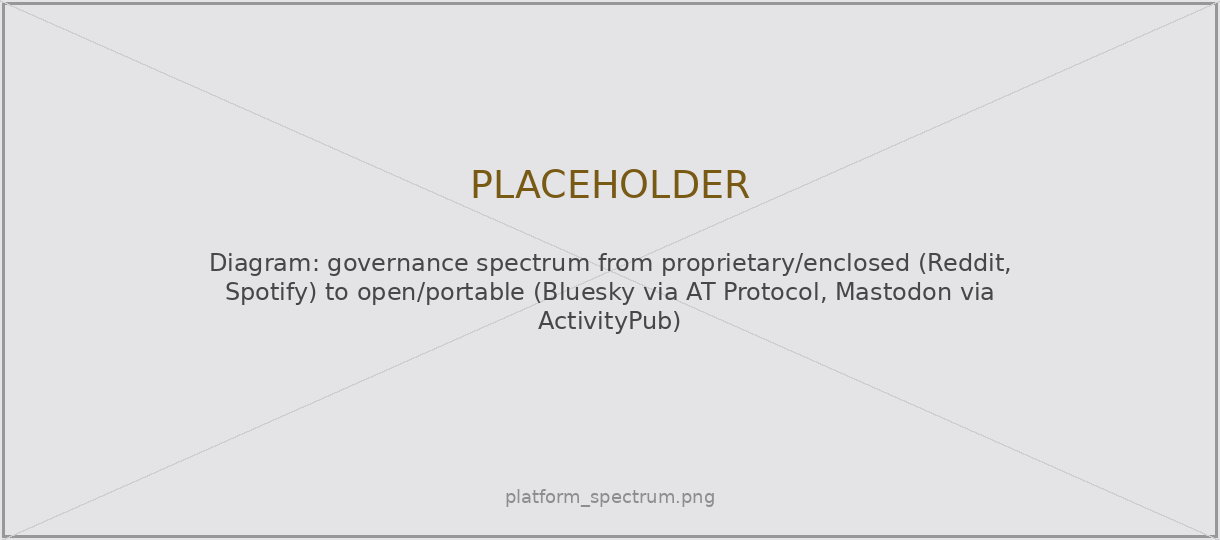
\includegraphics[width=\textwidth]{img/platform_spectrum.png}\\
            {\scriptsize Proprietary to open: who controls access.}
        \end{column}
    \end{columns}
    \bottomcite{Textbook Ch.~12, ``Platforms, Data, and Power.'' Cross-refs: Government APIs (Ch.~11), the post-API age (Ch.~2).}
\end{frame}

\begin{frame}{OAuth2: credentials for a scoped, revocable token}
    \begin{columns}[T]
        \begin{column}{0.54\textwidth}
            Almost every platform API authenticates with \textbf{OAuth2}. The idea: don't send your password with each request --- exchange your app's credentials for a \textit{scoped}, \textit{revocable} token.

            \vspace{0.8em}

            Two flows you should recognize:
            \begin{itemize}
                \item \textbf{Client credentials} --- authenticates the \textit{application}; grants read-only access to public data. Enough for research collection.
                \item \textbf{Authorization code} --- additionally asks a \textit{user} to grant your app permission to act for them. Every ``Sign in with Google'' dialog.
            \end{itemize}

            \vspace{0.6em}

            Store client IDs and secrets in environment variables, \textbf{never} in the notebook.
        \end{column}
        \begin{column}{0.42\textwidth}
            \centering
            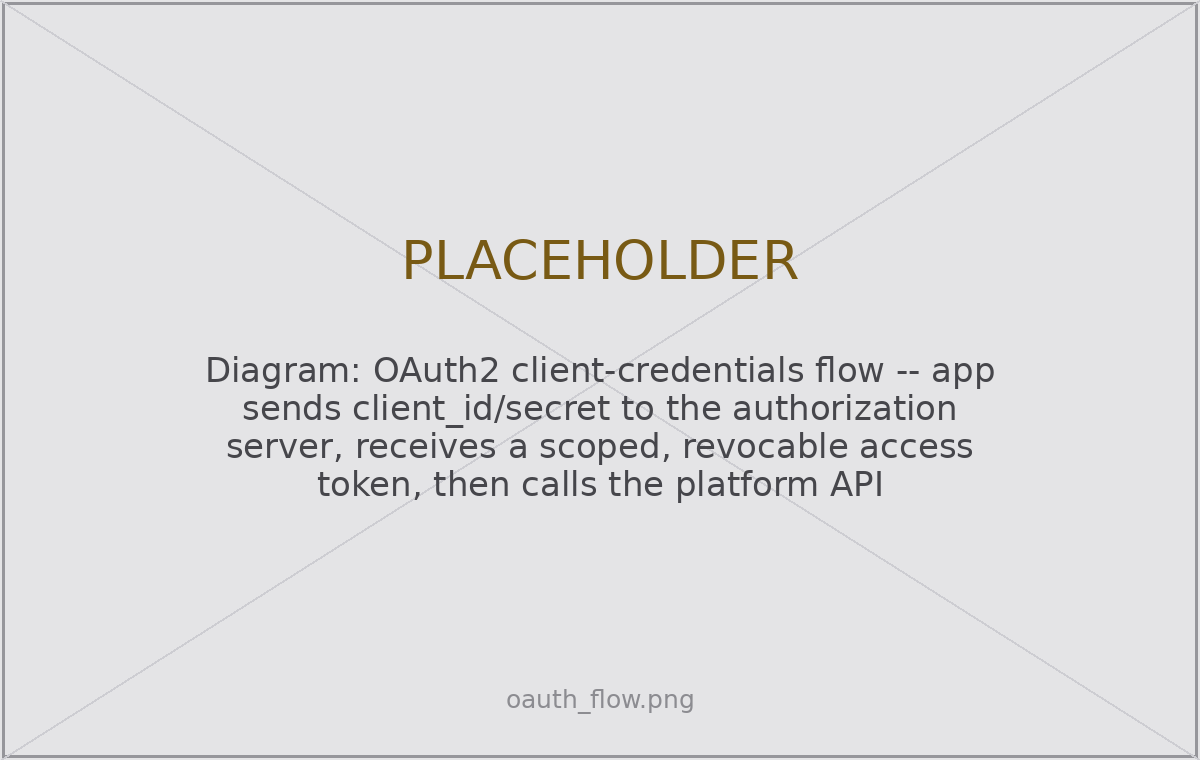
\includegraphics[width=\textwidth]{img/oauth_flow.png}\\
            {\scriptsize Bluesky app passwords and Mastodon tokens are the same delegated-credential idea, implemented more simply.}
        \end{column}
    \end{columns}
    \bottomcite{Textbook Ch.~12, ``Authentication.'' Credential hygiene: \textit{Missing Manual} Ch.~34.}
\end{frame}

\begin{frame}{Four platforms, four architectures}
    The differences are not cosmetic --- they decide what data exists, on what terms, and how durable your access is:
    \vspace{0.6em}

    \centering
    \footnotesize
    \begin{tabular}{@{}lllll@{}}
        \toprule
        \textbf{Platform} & \textbf{Protocol} & \textbf{Auth} & \textbf{Rate limit} & \textbf{Data ownership}\\
        \midrule
        Reddit   & Proprietary REST & OAuth2                & 100 QPM            & Platform-controlled\\
        Spotify  & Proprietary REST & OAuth2 / client creds & $\sim$180 RPM      & Platform-controlled\\
        Bluesky  & AT Protocol \textit{(open)}  & App password  & Generous, per-PDS  & \textbf{User-portable}\\
        Mastodon & ActivityPub \textit{(open)}  & OAuth2, per-instance & Varies      & Instance-governed\\
        \bottomrule
    \end{tabular}

    \vspace{0.9em}
    \raggedright
    Reddit and Spotify can \textit{unilaterally} rewrite their terms because they own both the platform \textbf{and} the protocol. Bluesky and Mastodon cannot --- their protocols are open standards anyone can implement. That is the architectural embodiment of \textbf{ownership} (Ch.~2).
    \bottomcite{Textbook Ch.~12, ``Comparing Platform Architectures.''}
\end{frame}

\begin{frame}{What the notebook covers}
    One authentication-to-DataFrame pattern, four times over:
    \begin{itemize}
        \item \textbf{Reddit (PRAW)} --- subreddit metadata, submissions, comment trees, depth-vs-engagement
        \item \textbf{Spotify (spotipy)} --- search, artist profiles, top-track popularity, user playlists
        \item \textbf{Bluesky (atproto)} --- author feeds and the social graph (followers, following, mutuals)
        \item \textbf{Mastodon (Mastodon.py)} --- public timelines, account search, and hashtags \textit{across} instances
    \end{itemize}
    Every one: \textbf{authenticate $\rightarrow$ request $\rightarrow$ parse nested JSON $\rightarrow$ DataFrame}.

    \vspace{0.8em}

    \begin{alertblock}{Connecting to Ch.~2 (Ethics): social data is people data}
        \footnotesize Every post, comment, and listening pattern was produced by a person who never imagined a research dataset. Check the ToS, consider IRB, collect the \textit{minimum} you need, never touch private or DM content, and don't quote posts in ways a search engine can re-identify.
    \end{alertblock}
\end{frame}

% =========================================================================
\section{Wednesday · Notebook Lab}
% =========================================================================

\begin{frame}[fragile]{Reddit via PRAW --- authenticate \& explore}
    Client-only credentials put PRAW in read-only mode --- exactly what research collection needs:
\begin{lstlisting}
import praw

reddit = praw.Reddit(
    client_id="your_client_id",
    client_secret="your_client_secret",
    user_agent="WebDataScience/1.0 by u/your_username")
print(reddit.read_only)               # True with app-only credentials

subreddit = reddit.subreddit("news")
print(f"Subscribers: {subreddit.subscribers:,}")
for rule in subreddit.rules:          # PRAW returns Rule objects
    print("-", rule.short_name)
\end{lstlisting}
    \bottomcite{Textbook Ch.~12, ``Reddit via PRAW.'' Free tier: 100 queries/minute for non-commercial use.}
\end{frame}

\begin{frame}[fragile]{Reddit --- comment trees \& the depth-decay pattern}
    \begin{columns}[T]
        \begin{column}{0.56\textwidth}
\begin{lstlisting}
sub = next(subreddit.hot(limit=1))
sub.comments.replace_more(limit=0)  # flatten tree

rows = [{"score": c.score,
         "depth": c.depth,
         "words": len(c.body.split())}
        for c in sub.comments.list()]
df = pd.DataFrame(rows)

df.groupby("depth")["score"].mean()
# decays sharply as nesting deepens
\end{lstlisting}
        \end{column}
        \begin{column}{0.42\textwidth}
            \centering
            
\includegraphics[width=\textwidth]{img/reddit_depth_decay.png}\\
            {\scriptsize Depth 0 comments score highest.}

            \vspace{0.5em}
            \raggedright\footnotesize Not a measure of quality --- an artifact of interface design, where nested replies are progressively collapsed and harder to reach.
        \end{column}
    \end{columns}
    \bottomcite{Textbook Ch.~12, ``Analyzing Comment Engagement.'' Score is skewed --- prefer a Spearman rank correlation.}
\end{frame}

\begin{frame}[fragile]{Spotify via spotipy --- search \& artist profile}
    The client-credentials flow reaches public catalog data --- artists, albums, tracks, user playlists:
\begin{lstlisting}
import spotipy
from spotipy.oauth2 import SpotifyClientCredentials

auth = SpotifyClientCredentials(client_id="...", client_secret="...")
sp = spotipy.Spotify(auth_manager=auth)

results = sp.search(q="Queen", type="artist", limit=1)
artist = results["artists"]["items"][0]
top = sp.artist_top_tracks(artist["id"])["tracks"]
print(artist["name"], f'{artist["followers"]["total"]:,}',
      [t["popularity"] for t in top[:5]])   # popularity is 0-100
\end{lstlisting}
    \bottomcite{Textbook Ch.~12, ``Spotify via spotipy.'' \texttt{popularity} is engagement-weighted and recomputed on Spotify's schedule.}
\end{frame}

\begin{frame}{The audio features story --- enclosure in miniature}
    \begin{columns}[T]
        \begin{column}{0.56\textwidth}
            For a decade the API's signature research offering was \textbf{audio features} --- danceability, energy, valence, tempo for every track. Hundreds of studies mapped genres and modeled hits with them.

            \vspace{0.7em}

            November 2024: cut off for all newly created apps. No stated research alternative --- just as generative AI made music data newly valuable.

            \vspace{0.7em}

            The lasting lesson: those scores were never ground truth. They were Spotify's \textit{proprietary model} of what music \textit{is}. You always analyze the platform's model of the world as much as the world itself.
        \end{column}
        \begin{column}{0.4\textwidth}
            \centering
            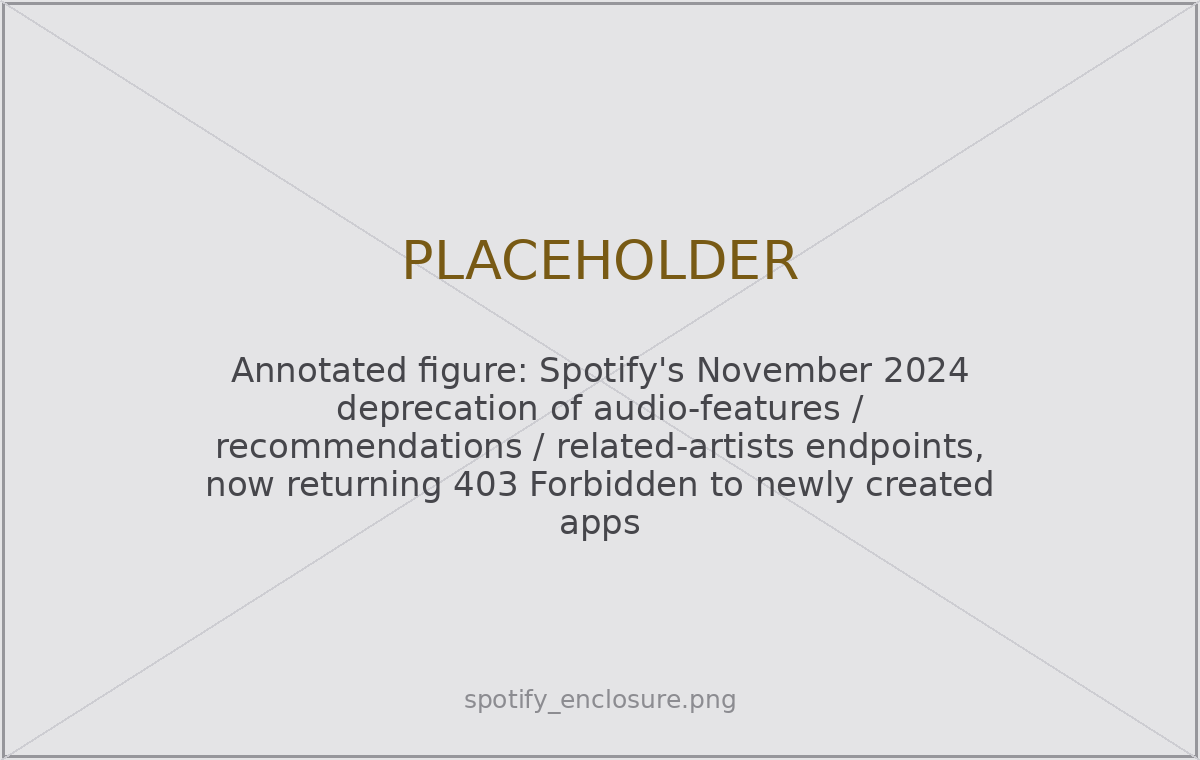
\includegraphics[width=\textwidth]{img/spotify_enclosure.png}
            \begin{alertblock}{A shrinking API}
                \footnotesize New apps get \texttt{403 Forbidden} on audio features, recommendations, and related artists. It is not a bug in your code --- the access no longer exists.
            \end{alertblock}
        \end{column}
    \end{columns}
    \bottomcite{Textbook Ch.~12, ``The Audio Features Story.'' Enclosure \& the post-API age (Ch.~2).}
\end{frame}

\begin{frame}[fragile]{Bluesky via the AT Protocol --- open by design}
    \begin{columns}[T]
        \begin{column}{0.57\textwidth}
\begin{lstlisting}
from atproto import Client

client = Client()
client.login("you.bsky.social",
             "your-app-password")

feed = client.app.bsky.feed.get_author_feed(
    {"actor": "bsky.app", "limit": 50})

posts = [{"text": i.post.record.text,
          "likes": i.post.like_count,
          "reply": i.post.record.reply is not None}
         for i in feed.feed]
df = pd.DataFrame(posts)
\end{lstlisting}
        \end{column}
        \begin{column}{0.4\textwidth}
            \centering
            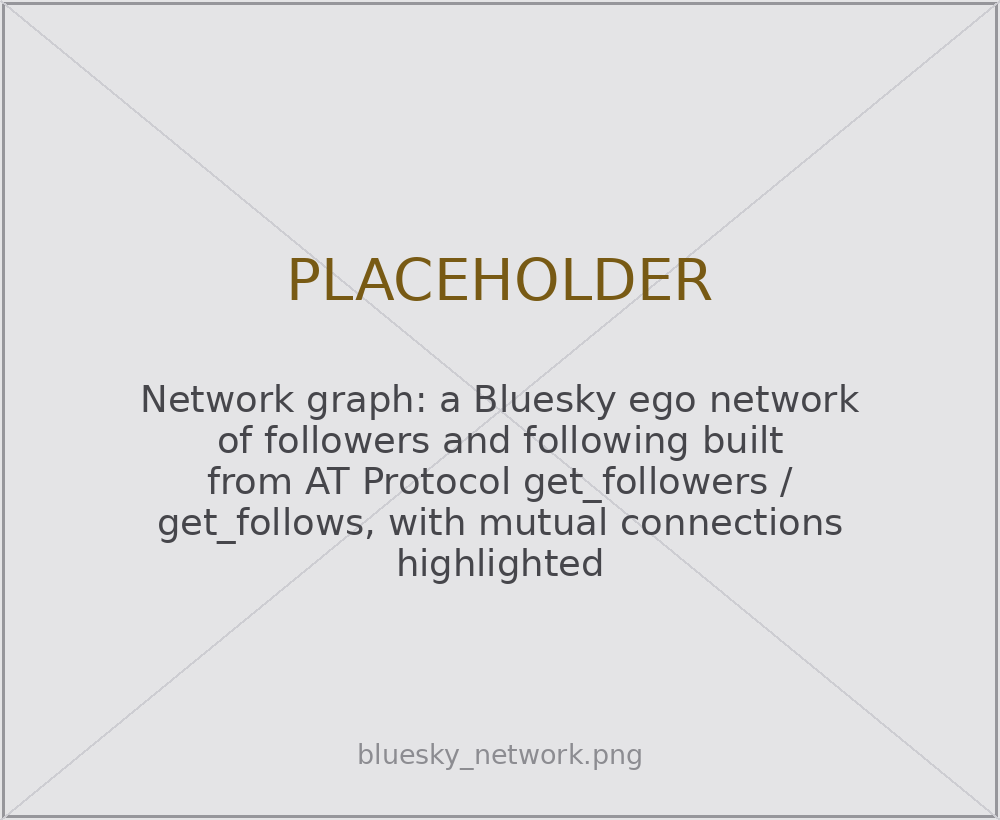
\includegraphics[width=0.92\textwidth]{img/bluesky_network.png}\\
            {\scriptsize Social graph via \texttt{get\_followers} / \texttt{get\_follows}.}

            \vspace{0.4em}
            \raggedright\footnotesize An \textbf{app password} is a revocable delegated credential --- OAuth's principle, simpler. Identity and graph are portable across any AT-Protocol service.
        \end{column}
    \end{columns}
    \bottomcite{Textbook Ch.~12, ``Bluesky via AT Protocol.'' No single company controls access.}
\end{frame}

\begin{frame}[fragile]{Mastodon via Mastodon.py --- federated, per-instance}
    Each instance runs its own API --- there is no single endpoint for ``all of Mastodon.'' Statuses arrive as HTML, so strip tags before analysis:
\begin{lstlisting}
from mastodon import Mastodon
from bs4 import BeautifulSoup

mastodon = Mastodon(access_token="user_cred.secret",
                    api_base_url="https://mastodon.social")

for toot in mastodon.timeline_public(limit=10):
    text = BeautifulSoup(toot["content"], "html.parser").get_text()
    print("@" + toot["account"]["username"], text[:80])

tagged = mastodon.timeline_hashtag("datascience", limit=20)
\end{lstlisting}
    Comprehensive collection means engaging \textit{many} instances --- each with its own rules, rate limits, and moderation norms.
    \bottomcite{Textbook Ch.~12, ``Mastodon via Mastodon.py'' \textcite{diener2026mastodonpy}. Built on ActivityPub.}
\end{frame}

\begin{frame}{Lab: work these, then show-and-tell}
    \begin{columns}[T]
        \begin{column}{0.62\textwidth}
            Register your own apps, then work in pairs:
            \begin{enumerate}\small
                \item Reddit: compare two subreddits on one topic (r/science vs.\ r/askscience) --- submissions, engagement, moderation
                \item Spotify: analyze an artist's full discography --- how has release cadence and back-catalog popularity shifted?
                \item Open vs.\ closed: pull a profile, graph, and posts from \textit{both} Bluesky and Reddit; compare ease and richness
                \item Playlist fingerprints: two user-created playlists, overlapping metadata distributions
                \item Bluesky: 50 posts via \texttt{get\_author\_feed} --- summary stats \& AT-Protocol limits
                \item[6.] \textcolor{tab-purple}{\textbf{5617}}: design a cross-platform measurement plan (proprietary vs.\ federated) --- \textcite{bruns2019after}, \textcite{davidson2023platform}
            \end{enumerate}
        \end{column}
        \begin{column}{0.34\textwidth}
            \begin{block}{Show-and-Tell}
                \footnotesize Come ready to share:
                \begin{itemize}\footnotesize
                    \item a challenging bug
                    \item interesting data you pulled
                    \item a provocation for a research design
                \end{itemize}
            \end{block}
        \end{column}
    \end{columns}
\end{frame}

\begin{frame}[standout]
    Platform goodwill is not infrastructure.\\[0.6em]
    Twitter went from the most important data source in\\
    computational social science to inaccessible --- in a year.\\[1em]
    {\large Build across open \emph{and} closed, so no single\\ shutdown ends your research.}
\end{frame}

% =========================================================================
\section{Friday · Textbook Revisions}
% =========================================================================

\begin{frame}{Improving Chapter 12 together}
    \begin{columns}[T]
        \begin{column}{0.6\textwidth}
            Today we make the book better. Each of you opens a \textbf{pull request} against \texttt{ch-12-social.qmd} and reviews a classmate's.

            \vspace{1em}

            The workflow (from Week 1):
            \begin{enumerate}\small
                \item Branch / fork the book repo
                \item Edit the chapter; commit with a clear message
                \item Open a PR describing \textit{what} and \textit{why}
                \item Review two peers' PRs: kind, specific, actionable
            \end{enumerate}

            \vspace{0.8em}

            \footnotesize This chapter drifts \textit{fast} --- endpoints and rate limits change --- so ``test it against the live API'' is unusually valuable here.
        \end{column}
        \begin{column}{0.36\textwidth}
            \centering
            
\includegraphics[width=\textwidth]{img/pr_review.png}
        \end{column}
    \end{columns}
    \bottomcite{Contributions \& reviews count toward the Textbook Revisions grade (30\%).}
\end{frame}

\begin{frame}{A revision menu for Chapter 12}
    High-value targets --- pick one and scope it to a single PR:
    \begin{itemize}
        \item \textbf{Test the code against live APIs.} Register an app, run the notebook, and report what broke: a Spotify \texttt{403}, a changed \texttt{atproto} method, a new rate limit. Fix it and note the date.
        \item \textbf{Close a gap in ``Common Issues to Debug.''} Add a worked PRAW \texttt{OAuthException} fix, a Mastodon instance-block/rate-limit case, or the \texttt{403}-diagnosis flowchart.
        \item \textbf{Add a figure.} An OAuth token-flow diagram, the governance-spectrum figure, or a clean comment depth-vs-score chart.
        \item \textbf{Strengthen a thin exercise.} The Bluesky and playlist exercises need expected output, a rubric, or starter cells so they are self-checking.
        \item \textbf{Refresh the comparison table \& ``Further Reading.''} Verify mid-2026 rate limits and endpoint availability; add a Fediverse-measurement paper tied to the \textbf{ownership} callout.
    \end{itemize}
    \bottomcite{Targets drawn from the chapter's callouts, ``Common Issues,'' thin exercises, and ``Further Reading.''}
\end{frame}

\begin{frame}{What makes a good revision \& a good review}
    \begin{columns}[T]
        \begin{column}{0.48\textwidth}
            \begin{block}{A strong PR}
                \begin{itemize}\small
                    \item One focused change, clearly titled
                    \item Explains the problem it fixes
                    \item Builds (\texttt{quarto render}) without errors
                    \item Matches the book's voice and notation
                    \item Discloses any AI assistance
                \end{itemize}
            \end{block}
        \end{column}
        \begin{column}{0.48\textwidth}
            \begin{block}{A strong review}
                \begin{itemize}\small
                    \item Runs / reads the change, not just skims
                    \item Names specifics (line, claim, code)
                    \item Separates ``must fix'' from ``nice to have''
                    \item Is generous --- assume good faith
                    \item Ends with a clear verdict
                \end{itemize}
            \end{block}
        \end{column}
    \end{columns}
    \vspace{0.5em}
    \centering\small Next week: \textbf{AI \& Language-Model APIs} --- sending prompts to models as one more data pipeline.
\end{frame}

% =========================================================================
\begin{frame}{Key takeaways}
    \begin{enumerate}
        \item One pattern, every platform: \textbf{authenticate $\rightarrow$ request $\rightarrow$ parse nested JSON $\rightarrow$ DataFrame}.
        \item OAuth2 trades credentials for a \textbf{scoped, revocable token}; client-credentials is enough for public research reads.
        \item The real variable is \textbf{governance}, not code: who owns the data, on what terms, and what happens when the rules change.
        \item Open protocols (AT, ActivityPub) make access an \textbf{architectural feature}; proprietary APIs make it a revocable business decision.
        \item Access is conditional, costly, and fragile --- build across open \textbf{and} closed so no single closure ends your research.
    \end{enumerate}
    \vspace{1em}
    \bottomcite{Reading: Textbook Ch.~12. Related: \textcite{baumgartner2020pushshift}; \textcite{diener2026mastodonpy}; \textcite{bruns2019after}.}
\end{frame}

\end{document}
